\documentclass[10pt]{article}
\usepackage{../../local}
\urlstyle{same}

\newcommand{\classcode}{EE 120}
\newcommand{\classname}{Signals and Systems}
\renewcommand{\maketitle}{%
\hrule height4pt
\large{Eric Du \hfill \classcode}
\newline
\large{HW 04} \Large{\hfill \classname \hfill} \large{\today}
\hrule height4pt \vskip .7em
\small{Header styling inspired by CS 70: \url{https://www.eecs70.org/}}
\normalsize
}
\linespread{1.1}

\newcommand{\corr}{\mathrm{corr}}
\newcommand{\sinc}{\mathrm{sinc}}
\begin{document}
	\maketitle
	\section*{Collaborators}
	I worked with the following people to complete this assignment:
	\begin{itemize}
		\item Teja Nivarthi: 3036508567
		\item Nikhil Maserang: 3036978230
	\end{itemize}
	\pagebreak
	\section*{Problem 1}
	An important concept in many communications applications is the correlation between two signals. This problem 
	is meant to serve as a brief introduction to correlation functions and some of their properties. 

	Let \( x(t) \) and \( y(t) \) be two signals; then the \textit{correlation function} is defined as 
	\[
	r_{xy}(t) = (x \circ y)(t) = \corr(x, y) = \int_{-\infty}^{\infty} x(\tau) y(t + \tau) \diff \tau 
	\] 
	The function \( r_{xx} \) is usually referred to as the \textit{autocorrelation function} of the signal \( x(t) \), 
	while \( r_{xy}(t) \) is often called a \textit{cross-correlation function}. 
	\begin{enumerate}[label=\alph*)]
		\item What is the relationship between \( r_{xy}(t) \) and \( r_{yx}(t) \)?

			\begin{solution}
				We can write \( r_{yx}(t) \) as:
				\[
				r_{yx}(t) = \int_{-\infty}^{\infty} y(\tau) x(t + \tau)\diff \tau 
				\] 
				Now, let \( \tau' = t + \tau \), meaning that \( \tau = \tau' - t \). Therefore:
				\[
				r_{yx}(t) = \int_{-\infty}^{\infty} x(\tau') y(-t + \tau') \diff \tau' 
				\] 
				This is the same as \( r_{xy}(t) \), except that we now have \( -t \) instead of \( t \). Therefore, 
				the relationship is:
				\[
				r_{xy}(t) = r_{yx}(-t)
				\] 
			\end{solution}
		\item Compute the odd portion of \( r_{xx}(t) \). 

			\begin{solution}
				We will begin by using the property that the odd part of any function can be written as:
				\[
				f_o(t) = \frac{f(t) - f(-t)}{2}
				\] 
				Applying this to our autocorrelation function:
				\[
					r_{xx, o}(t) = \frac{r_{xx}(t) - r_{xx}(-t)}{2} 
				\]
				Then, from part (a) we know that \( r_{xx}(t) = r_{xx}(-t) \), so this actually just becomes 0. 
			\end{solution}
		\item Suppose that \( y(t) = x(t + T) \). Express \( r_{xy}(t) \) and \( r_{yy}(t) \) in terms of 
			\( r_{xx}(t) \). 

			\begin{solution}
				We have:
				\begin{align*}
					r_{xx}(t) &= \int_{-\infty}^{\infty} x(\tau) x(t + \tau) \diff \tau  \\
					r_{xy}(t) &= \int_{-\infty}^{\infty} x(\tau) y(t + \tau) \diff  \tau = \int_{-\infty}^{\infty} 
					x(\tau) x(t + \tau + T) \diff \tau\\
					r_{yy}(t) &=  \int_{-\infty}^{\infty} y(\tau) y(t + \tau) \diff \tau = 
					\int_{-\infty}^{\infty} x(\tau + T) x(t + \tau + T) \diff \tau 
				\end{align*}
				Notice that for \( r_{xy}(t) \), this is the same equation as \( r_{xx}(t) \) but with 
				\( t + T \) as an input. Therefore, we have \( r_{xy}(t) = r_{xx}(t + T) \). For 
				\( r_{yy}(t) \), let \( \tau' = \tau + T \), then we can write:
				\[
				r_{yy}(t) = \int_{-\infty}^{\infty} x(\tau')x(t + \tau') \diff \tau' 
				\] 
				which is the same integral as \( r_{xx}(t) \), so we conclude that \( r_{yy}(t) = r_{xx}(t)  \).
			\end{solution}
	\end{enumerate}
	\pagebreak
	\section*{Problem 2}
	\begin{enumerate}[label=\alph*)]
		\item \textbf{One-sided decaying potential:} The CTFT of the one-sided decaying exponential \( x(t) = 
			e^{-at} u(t), \forall t\), where \( a >0 \in \R \) is given by 
			\[
				\mathcal F\{x(t)\} = X(\omega) = \frac{1}{a + i \omega}
			\] 
			as shown in discussion and lecture. Provide a well-labeled sketch of \( |X(\omega)|, \forall \omega \). 
			Describe how the bandwidth of \( x \) varies in relation to the decay rate \( a \) of the one-sided
			potential?

			\textit{Note:} Consider as the bandwidth frequency \( \omega_B \) the threshold where 
			\( |X(\omega_B) = \frac{1}{\sqrt{2} }\max_\omega |X(\omega)| \). This bandwidth frequency (or cutoff 
			frequency) is chosen by convention to correspond to the "3 dB (decibel)" drop in magnitude. Notice that 
			\( 20 \log_{10}(\frac{1}{\sqrt{2} }) \approx -3 \text{ dB} \). This has historical roots in circuit 
			theory and design. 

			\begin{solution}
				We can write:
				\[
				|X(\omega)| = \frac{1}{\sqrt{a^2 + \omega^2} }
				\] 
				For \( a =1 \), the plot looks like this: 
				\begin{center}
					\includegraphics[scale=0.8]{q2a1.png}
				\end{center}
				For \( a = 10 \), the plot looks like this:
				\begin{center}
					\includegraphics[scale=0.8]{q2a2.png}
				\end{center}
				What we can see is that the peak of \( |X(\omega)| \) shrinks considerably, but the signal also 
				takes much longer to decay. This is evidenced by the fact that at for 
				\( a = 1 \), \( |X(\omega)| \) is almost zero at \( \omega = 10 \), whereas it is roughly 
				0.0075 when \( a = 10 \). The bandwidth therefore increases as \( a \) increases. 

				Intuitively this also makes sense. As \( a \) increases, then \( |X(\omega)| \) depends less 
				on \( \omega \) for small values of \( \omega \). In other words, when \( a \) is larger, then 
				\( \omega \) needs to also be larger in order for us to see the effects of \( \omega \) in 
				\( |X(\omega)| \). Thus, there is less \( \omega \) dependence at small \( \omega \), therefore 
				the bandwidth increases. 
			\end{solution}
		\item For this and all following signals, determine \( X(\omega) \), their corresponding continuous-time 
			Fourier transform (CTFT). \\
			\textbf{Two-sided decaying exponential:} \( x(t) = e^{-a|t|}, \forall t \), where \( a >0 \). 

			\begin{solution}
				We solve this in almost the identical way to problem 1.2b:
				\begin{align*}
					X(\omega) &= \int_{-\infty}^{\infty} e^{-a|t|}e^{-i \omega t}\diff t \\
					&= \int_{-\infty}^{0} e^{at}e^{-i \omega t}\diff t + \int_{0}^{\infty} e^{-at} e^{-i \omega t}
					\diff t\\
					&= \frac{1}{a - i \omega}e^{(a - i \omega) t} \biggr|{-\infty}^0 
					- \frac{1}{a + i \omega}e^{-(a + i \omega) t}\biggr|_0^\infty\\
					&= \frac{1}{a - i \omega} + \frac{1}{a + i \omega} \\
					&= \frac{2a}{a^2 + \omega^2} 
				\end{align*}
				This aligns exactly with the solution to 1.2b, since we have te condition that \( a > 0 \) here 
				(since we have \( e^{-a|t|} \) instead of \( e^{a|t|} \) that we had in 1.2b.)
			\end{solution}
		\item \textbf{Sinusoid:} \( x(t) = \sin(\omega_0 t), \forall t \). \\
			\textit{Hint:} It may be helpful to decompose the signal into complex exponentials using Euler's 
			formula. 

			\begin{solution}
				We follow the hint, and use the fact that \( \sin(\omega_0t) = \frac{1}{2i}(e^{i \omega_0 t}
				- e^{-i \omega_0t})\). Therefore:
				\begin{align*}
					X(\omega) &= \frac{1}{2i}\left[ \int_{-\infty}^{\infty} e^{i \omega_0 t - i \omega t}
					- e^{-i \omega_0 t - i \omega t} \diff  t\right]  \\
					&= \frac{1}{2i}(\delta(\omega - \omega_0) - \delta(\omega + \omega_0)) 
				\end{align*}
				This makes sense -- the Fourier transform of a pure sine wave is just a linear combination of 
				the left-travelling and right-travelling wave at frequency \( \omega_0 \).
			\end{solution}
	\end{enumerate}
	\pagebreak
	\section*{Problem 3}
	\begin{enumerate}[label=\alph*)]
		\item Calculate the CTFT of a finite-duration rectangular signal of arbitrary width and length. 
			\[
			x(t) = \begin{cases}
				b & |t| \le a\\
				0 & \text{otherwise}
			\end{cases}
			\] 
			Describe how the CTFT of this signal changes as the parameters \( a \) and \( b \) change. You can 
			assume that the parameters \( a \) and \( b \) have appropriately-chosen positive values. Experss your 
			final answer as an expression involving a sinc function defined as
			\[
			X(\omega) = \sinc(\omega) = \begin{cases}
				\frac{\sin(\pi \omega)}{\pi \omega} & \text{if \( t \neq 0 \)}\\
				1 & \text{if \( t =0 \)}
			\end{cases}
			\] 
			\textit{Note:} As a sanity check and a bit of background for part (b), the solution to this problem 
			should demonstrate a phenomenon known as the time-frequency uncertainty principle. This principle 
			states that a given function cannot be arbitrarily compact in both time and frequency. Practically 
			what this means is that as you shrink (define using fewer timesteps) the time-domain representation, 
			the number of frequencies defining your impulse response will increase (frequency spectrum will widen), 
			and vice versa. 

			\begin{solution}
				Here we just take the Fourier transform:
				\begin{align*}
					X(\omega) &=  \int_{-\infty}^{\infty} x(t) e^{-i \omega t}\diff  t  \\
					&= \int_{-a}^{a} be^{-i \omega t}\diff t  \\
					&= -\frac{b}{i \omega}\left[ e^{-i \omega t} \right]_{-a}^{a} \\
					&= -\frac{b}{i \omega}\left[ e^{i \omega a} - e^{- i \omega a} \right]  \\
					&= \frac{2b}{\omega}\sin(\omega a) 
				\end{align*}
				Then, using the property of the sinc function, we can see that: 
				\[
				\sinc\left( \frac{\omega a}{\pi} \right) = \frac{\sin(\omega a)}{\omega a}
				\] 
				So we can write:
				\[
				X(\omega) = 2ab \sinc\left( \frac{\omega a}{\pi} \right) 
				\] 
			\end{solution}
		\item We call a signal bandlimited (in frequency) if \( \exists B_1 \le B_2 \in \R \) such that 
			\( \forall \omega \le  B_1, \omega \ge B_2, X(\omega) = 0 \). Likewise, we call a signal finite duration
			(in time) if there \( \exists T_1 \le  T_2 \in \R \) such that \( \forall t \le  T_1, t >T_2, x(t) = 0 \). 
			Show that if a signal has finite duration, then it is not bandlimited. You can ignore the trivial case 
			of \( x(t) = 0 \). Explain why this is a manifestation of the time-frequency uncertainty principle. 

			\textit{Hint:} It is possible to re-express \textbf{any} finite-duration or band-limited signal 
			in terms of the familiar box we have been working with. 

			\begin{solution}
				We can always write a finite duration signal as a product of a rectangular box of height 1 
				and a (potentially infinite) signal \( f(t) \):
				\[
				x(t) = f(t) \cdot \sqcap(t)
				\] 
				Then, we have to take the Fourier transform of this. Using the convoluiton theorem, we have:
				\[
				X(\omega) = \mathcal F \{f(t)\} * \mathcal F \{\sqcap(t)\} 
				\] 
				We know the convolution of the square pulse is a sinc function, which is not band limited (part a). 
				Then, 
				since the width of functions is additive in a convolution, then since \( \mathcal F \{\sqcap(t)\}  \) 
				is not band limited then the entire transform \( X(\omega) \) is also not band limited. 

				This is a manifestation of the time-frequency uncertainty principle, since it says that if we have 
				a localized function in time, then taking the Fourier transform gives us a function that isn't localized
				in frequency. 
			\end{solution}
	\end{enumerate}
	\pagebreak
	\section*{Problem 4}
	Consider the following impulse responses of two LTI systems: 
	\begin{align*}
		h(t) &= \delta(t - 2)\\
		g(t) &=  e^{-\alpha|t|}, \alpha \in \R+  
	\end{align*}
	\begin{enumerate}[label=\alph*)]
		\item Find \( H(\omega) \) and \( G(\omega) \), the frequency responses (CTFT) of the systems. 

			\begin{solution}
				We compute \( H(\omega) \) first:
				\begin{align*}
					H(\omega) &= \int_{-\infty}^{\infty} \delta(t - 2) e^{-i \omega t}\diff t  \\
					&= e^{- 2 i \omega} 
				\end{align*}
				For \( G(\omega) \), this is the same thing as problem 2b, so we can just use that result:
				\[
				G(\omega) = \frac{2\alpha}{\alpha^2 + \omega^2}
				\] 
				where \( \alpha >0 \). 
			\end{solution}
		\item Consider interconnected LTI systems with impulse responses \( h(t)  \) and \( g(t) \):
			System 1, with overall impulse response of \( s_1(t) \):
			\begin{center}
				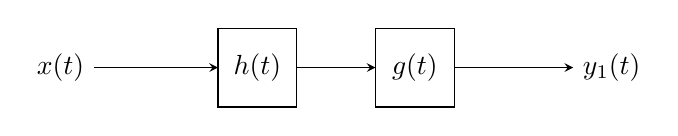
\begin{tikzpicture}
					\node (A) at (-3, 0) {\( x(t) \) };
					\node (B) at (4, 0) {\( y_1(t) \) };
					\draw[-stealth] (A) -- (-1, 0);
					\draw (-1, -0.5) rectangle node {\( h(t) \) } (0, 0.5);
					\draw[-stealth] (0, 0) -- (1, 0);
					\draw (1, -0.5) rectangle node { \( g(t) \) } (2, 0.5);
					\draw[-stealth] (2, 0) -- (B);
				\end{tikzpicture}
			\end{center}
			System 2, with overall impulse response of \( s_2(t): \)
			\begin{center}
				\begin{tikzpicture}
					\node (A) at (-3, 0) {\( x(t) \) };
					\node (B) at (4, 0) {\( y_2(t) \) };
					\node (C) at (1.5, 0) {+};
					\draw[-stealth] (A) -- (-0.5, 0) -- (-0.5, 1) -- (0, 1);
					\draw (0, 0.5) rectangle node {\( h(t) \) } (1, 1.5);
					\draw[-stealth] (-0.5, 0) -- (-0.5, -1) -- (0, -1);
					\draw (0, -0.5) rectangle node {\( g(t) \) } (1, -1.5);
					\draw[-stealth] (1, 1) -- (1.5, 1) -- (C);
					\draw (C) circle (0.2cm);
					\draw[-stealth] (C) -- (B);
					\draw[-stealth] (1, -1) -- (1.5, -1) -- (C);
				\end{tikzpicture}
			\end{center}

			Find the impulse responses \( s_1(t) \) and \( s_2(t) \). Also find their respective 
			frequency responses \( S_1(\omega) \) and \( S_2(\omega) \). 

			\begin{solution}
				Starting with system 1, since the impulse responses are connected in series, then we know that 
				the impulse response of the entire sytsem is given by the convolution of the two: 
				\[
				s_1(t) = h(t) * g(t) = \int_{-\infty}^{\infty} \delta(\tau - 2) e^{-\alpha |t - \tau|}
				\diff \tau = e^{-\alpha|t - 2|}
				\] 
				For system 2, the impulse response is the sum of \( h \) and \( g \), since the systems are connected
				in parallel:
				\[
				s_2(t) = h(t) + g(t) = \delta(t - 2) + e^{-\alpha|t|}
				\] 
				Now for \( S_1(\omega) \) and \( S_2(\omega) \). Since \( s_1(t) \) is a convolution of two 
				functions, then the convolution theorem says that the Fourier transform of it is going to be a 
				product of the two transformed functions. That is, 
				\[
					S_1(\omega) = \mathcal F \{s_1(t)\} = \mathcal F \{h(t) * g(t)\}  = H(\omega) \cdot G(\omega)
					= \frac{2\alpha e^{-2 i \omega}}{\alpha^2 + \omega^2}
				\] 
				For \( S_2(\omega) \), we know that the Fourier transform is linear, so:
				\[
				S_2(\omega) = \mathcal F \{s_2(t)\}  = \mathcal F \{h(t) + g(t)\}  = \mathcal F \{h(t)\}  + 
				\mathcal F \{g(t)\} = e^{-2 i \omega} + \frac{2\alpha}{\alpha^2 + \omega^2}
				\] 
			\end{solution}
		\item Now suppose 
			\[
			x(t) = e^{i \omega_0 t}
			\] 
			Calculate the output \( y(t) \) of the two systems \( S_1 \) and \( S_2 \) when given 
			\( x(t) \) as an input. 

			\textit{Hint:} Convert \( x(t) \) to the frequency domain, and feed it through the composite system 
			before taking the inverse transform of the result. As a further hint, note that the convolution in the 
			time domain is equivalent to multiplication in the frequency domain.

			\begin{solution}
				For system 1, we apply the hint and convert into the frequency domain. The Fourier transform 
				of \( x(t) \) is \( X(\omega) = \delta(\omega - \omega_0) \). Then, since we know that the 
				system output is characterized by a convolution, then the convolution theorem makes this especially 
				easy: 
				\[
				Y(\omega) =\mathcal F \{y(t)\}  = \mathcal F \{x(t)\} \cdot \mathcal F \{h(t)\} \cdot \mathcal F \{g(t)\} 
				= \delta(\omega - \omega_0)  \frac{2\alpha e^{-2 i \omega}}{\alpha^2 + \omega^2}
				\] 
				Then, we have to take the inverse Fourier transform of this in order to get back into 
				temporal space:
				\[
				y(t) = \mathcal F^{-1} \{Y(\omega)\}  = \frac{1}{2\pi}\int_{-\infty}^{\infty} 
				\delta(\omega - \omega_0) \frac{2\alpha e^{-2 i \omega}}{\alpha^2 + \omega^2} e^{i \omega t}\diff
				\omega = \frac{\alpha e^{-2 i \omega_0}}{\pi(\alpha^2 + \omega^2)} e^{ i \omega_0 t}
				\] 
				We'll use the same trick for system 2: 
				\[
				Y(\omega) = \mathcal F \{x(t)\}  \cdot \mathcal F \{s_2(t)\} = \delta(\omega - \omega_0) 
				\left( e^{-2 i \omega} + \frac{2\alpha}{\alpha^2 + \omega^2} \right) 
				\] 
				Then, we can take the inverse Fourier transform to get \( y(t) \):
				\[
				y(t) = \mathcal F^{-1} \{Y(\omega)\} = \frac{1}{2\pi}\int_{-\infty}^{\infty} 
				\delta(\omega - \omega_0)\left( e^{-2 i \omega} + \frac{2\alpha}{\alpha^2 + \omega^2} \right) 
				e^{i \omega t}\diff \omega = \left( e^{-2 i \omega_0} + \frac{2\alpha}{\alpha^2 + \omega_0^2} \right) 
				e^{i \omega_0t}
				\] 

			\end{solution}
	\end{enumerate}
\end{document}
